%%%%%%%%%%%%%%%%%%%%%%%%%%%%%%%%%%%%%%%%%%%%%%%%%%%%%%%%%%%%%%%%%%%%%%%%%%%%%%%%
%2345678901234567890123456789012345678901234567890123456789012345678901234567890
%        1         2         3         4         5         6         7         8
% THESIS Chapter

\chapter{Background theory}
\label{chap:relatedterms}
\ifpdf
    \graphicspath{{RelatedTerminology/Figures/PNG/}{RelatedTerminology/Figures/PDF/}{RelatedTerminology/Figures/}}
\else
    \graphicspath{{RelatedTerminology/Figures/EPS/}{RelatedTerminology/Figures/}}
\fi


% short summary of the chapter `` ''
% \section*{Summary}

% Describe here the state of the art of the research pertaining to this thesis. This part should contain all the relevant publications in the area with the corresponding citations. The cited works should be briefly described critically assessed.
%

Each type of information extracted from an audio stream is referred to as an
\textit{audio feature}. Audio features are mainly derived using various
transformations on the signal based on some basic properties of sound. They
allow for music data to be comparable and algorithmically accessible
\cite{mullershort}. This section presents low-level theory required to
understand the high-level description of how each feature is obtained further in
the report. At this level of the project description we only require an
understanding of general principles related to audio and signal processing,
therefore the explanations are kept concise without going deeper into technical
details.


\section{Basic properties of audio signal}
\label{sec:audioprops}
A \textit{digital audio signal} is a representation of the continuous sound wave
as a series of binary numbers. This representation helps preserve the
\textit{frequency} (the speed of the vibrations), as well as the
\textit{amplitude} (the fluctuations of the vibrations) of the sound. The energy
that each sound wave emits through vibrations is called \textit{sound energy}
and its rate is measured through \textit{sound power}. The majority of audio
features use frequency or power as a primary audio property used to define the
feature (\textit{modify/change}). 

\subsection{Sampling and sample rate}
\label{subsec:sampling}
The process of converting an analogue sound wave to a digital one involves a
process of extracting points (samples) from the continuous signal and using them
to describe the signal into a discrete form. This method is called
\textit{sampling} and the amount of samples collected per time frame is
\textit{sample rate}. The representation of a song used during feature
extraction is a sequence of samples extracted from the digital signal of the
song based on its sample rate.

\subsection{Tones}
\label{subsec:tones}
Western music is described using \textit{tones}, steady periodic sounds
\cite{wiki:tone}. They can be pure if the sound has sinusoidal waveform, or
complex if they are a combination of pure tones with a periodic repetition
pattern. Any of the waves contained in a complex tone is called a
\textit{partial}. The lowest of the tones determined by frequency is called a
\textit{fundamental}, with each of the tones higher than the fundamental defined
as \textit{overtones}. 

Tones are distinguished by several basic perceptual properties of sound - pitch,
loudness, timbre and duration \cite{acoustic-glossary-power}. A half tone is
called a \textit{semitone} and it is the smallest measure of period between
sounds. Semitones are grouped into \textit{octaves} where each octave contains
12 semitones. The acoustic opposite of tone is noise, a disordered sound which
is unpleasant to the human brain and is disruptive to hearing
\cite{music-noise}. 

\subsection{Psychoacoustic properties}
\label{subsec:psychoacoustic}
In order to understand how properties of a digital signal could form audio
features we first need to examine how they relate to the ways of how people
perceive music and sound. 

Several basic perceptual properties of sound are regularly used to describe what
is captured by each audio feature. They are pitch, loudness, timbre and
duration. Klapuri et al. \cite{klapuri2007signal} form good definitions of the
psychoacoustical terms outlined. They define \textit{pitch} as a perceptual
attribute which offers ordering of tones on a frequency-related scale. The term
is very closely related to tone and sometimes both definitions are used
interchangeably. Different pitches could be labelled through the Helmholz pitch
notation \cite{helmholtz2013sensations} using letters, through scientific pitch
notation \cite{fletcher1934loudness} utilising letters and numbers, or directly
using numbers representing the closest frequency in hertz (Hz). Despite being
determined by clear and stable frequencies in sound, pitch is more importantly a
subjective auditory sensation, so a strict mathematical relationship between
frequency and pitch does not exist \cite{acoustical1986american}. As a standard
it is accepted the musical note of A above C (Helmholz notation) or A4
(scientific notation) has a frequency of 440 Hz \cite{young1939terminology}. The
human ear perceives musical intervals on an approximately logarithmic scale with
respect to a \textit{fundamental frequency}, the lowest frequency available in a
tone and therefore determining the overall pitch of the tone. The set of sounds
with frequencies an integer multiple to the fundamental frequency is called
\textit{harmonic series} with every member of the set being a \textit{harmonic}.
In relation to this any partial with a frequency matching a harmonic is called a
\textit{harmonic partial}.

Using this notion of logarithmic perception there are various mappings of
pitches to frequencies, the most famous of which is the MIDI tuning standard
\cite{mts}.

Similar to tones, pitches are also ordered in octaves, where an octave is an
interval between one pitch and another with double its frequency
\cite{wiki:octave}. The set of all pitches which are within one octave of each
other is called a \textit{pitch class}.

\textit{Loudness} is another subjective psychoacoustical attribute of sound
\cite{klapuri2007signal}. Similar to how pitch is related to frequency, loudness
is a perception of sound pressure. \textit{Sound pressure} is a measurement of
the pressure divergence caused by a sound wave to the ambient atmospheric
pressure \cite{sound-pressure}. Loudness orders sounds on a scale ranging from
quiet to loud \cite{acoustical1986american}.

Tones also have a "colour" attribute attached to them through the introduction
of \textit{timbre}. Timbre allows distinguishing sounds with potentially
identical pitch, loudness and duration, but produced by different musical
instruments \cite{klapuri2007signal}. In large part this is determined by the
overtones in the sound generated alongside the fundamental frequency when a
musical instrument is played. While we already established that the fundamental
frequency determines the pitch of a tone, the added overtones create a more
complex and richer sound, they add "colour" to it. Overtones cannot be perceived
as separate notes, but we do hear them - they determine the timbre of an
instrument.

Timbre is a complex concept which cannot be defined by a single property of
sound. There are many attempts at breaking down the attribute into components.
Robert Erickson \cite{erickson1975sound} offers one of the most accepted
decompositions where timbre relates to the following acoustic parameters of
sound:
\begin{enumerate}
    \item Tonal and noise characters
    \item Time envelope - A \textit{time envelope} describes how sounds changes
    over time \cite{wiki:envelope}. It measures how much time it takes for the sound to reach an
    amplitude level when a musical instrument is activated (a key on the piano
    is pressed, for example) and subsequently how long it takes for the sound to
    go back to its initial level. 
    \item Spectral envelope and any changes to it - when only the curve of the
    amplitude out of a time envelope is taken into consideration then a
    \textit{spectral envelope} is used. Figures \ref{fig:time-envelope} and
    \ref{fig:spectral-envelope} illustrate the difference of between both envelopes.
    \item Changes in the fundamental frequency
    \item Onset dissimilar to the dominant vibration - with \textit{onset}
    being the start of a musical note we look for 'anomalies' in
    the vibration of the wave compared to the vibrations following the anomaly.

\end{enumerate}

\begin{figure}[H]
    \centering
    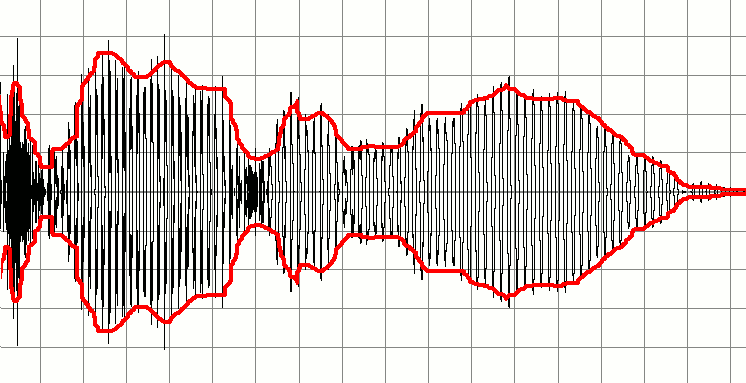
\includegraphics[width=0.75\textwidth]{BackgroundTheory/time_envelope.png}
    \captionof{figure}{Time envelope \textit{add citations and description}}
    \label{fig:time-envelope}
\end{figure}

\begin{figure}[H]
    \centering
    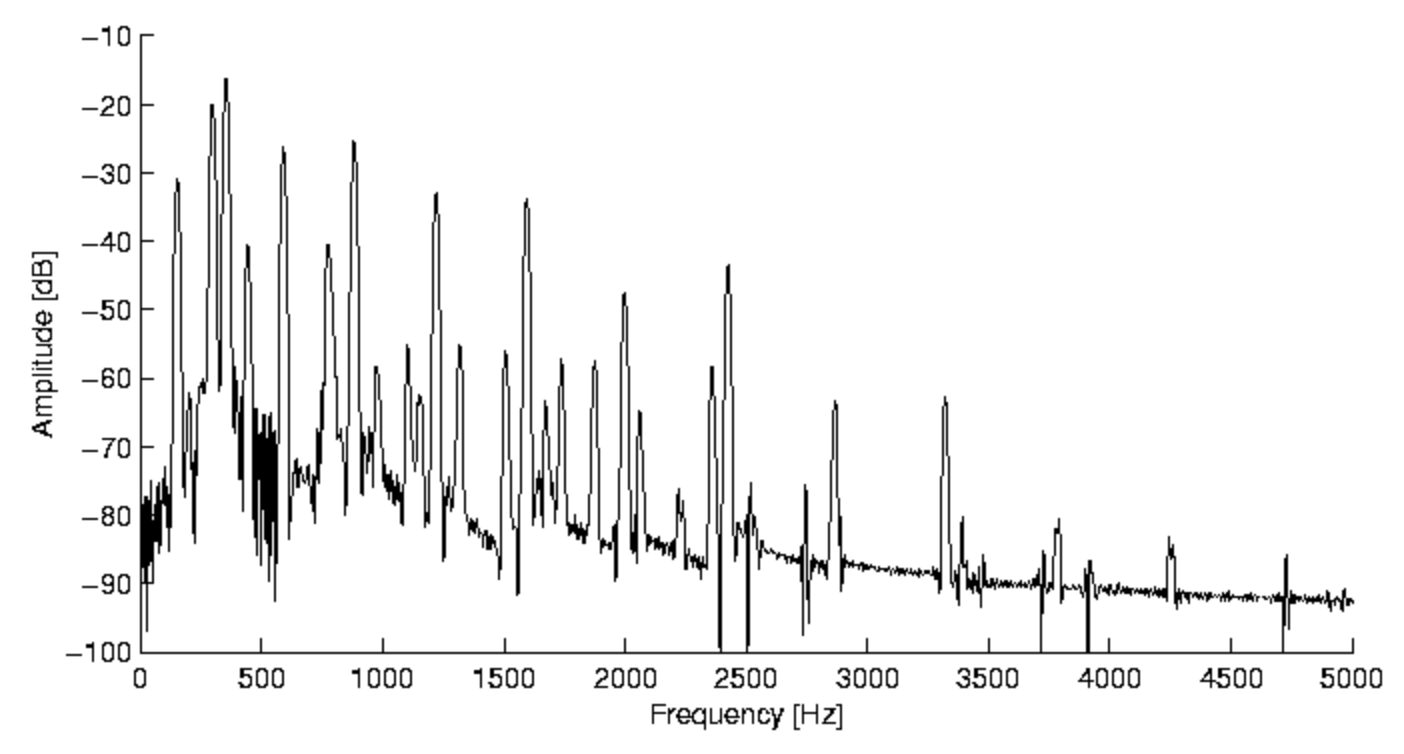
\includegraphics[width=0.75\textwidth]{BackgroundTheory/spectral_envelope}
    \captionof{figure}{Spectral envelope \textit{add citations and description}}
    \label{fig:spectral-envelope}
\end{figure}

Out of all psychoacoustical properties introduced \textit{duration} is the one
which is the easiest to directly measure. It is an indicator of a length of any
part of a musical composition - tone, pitch, the whole piece, etc
\cite{benward2014music}. The measurement is expressed using a base unit of time.

\subsection{Beat}
\label{subsec:beat}
One final basic concept that we need to introduce is the \textit{beat}. It
signifies repeating portions in a song which define the overall rhythm of a
music piece. Rhythm is formed of "strong" and "weak" beats, with the former
signifying a suitable moment for melody change.

\section{Audio transformation techniques}
\label{sec:audiotransform}

\subsection{Fourier transform}
\label{subsec:fourier}
Any waveform including the audio ones could be presented as a sum of sinusoids
of different frequencies \cite{fouriertransform}. In music each of the
constituting frequencies represents a pure tone. In order to be able to work
with the tonal representation of a song we need to perform \textit{Fourier
analysis}, that is, find a way to separate the different frequencies within the
audio signal. We achieve that using a decomposition called \textit{Fourier
transform} - one of the most widely used audio transformations.

\begin{figure}[H]
    \centering
    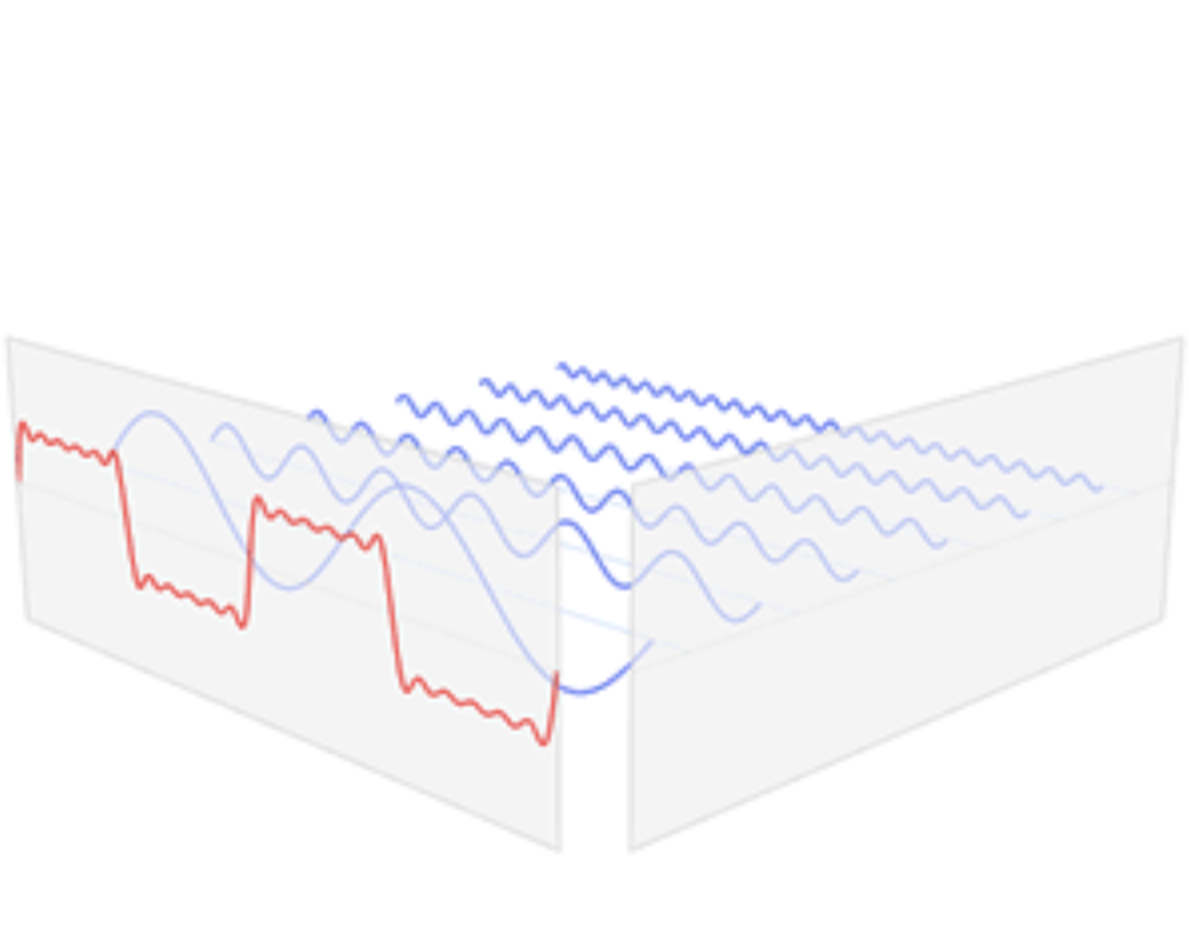
\includegraphics[width=0.75\textwidth]{BackgroundTheory/fourier-series.png}
    \captionof{figure}[Fourier transform applied on a periodic function]{Fourier transform applied on a periodical function (in red). The transform distinguishes six sine functions (in blue) represented as an amplitude-frequency relationship \cite{fourierseries}}
    \label{fig:fourierseriesimage}
\end{figure}

Fourier transform could be applied to either periodic (resulting in
\textit{Fourier series}) or non-periodic functions. As we are working in the
domain of music we are focussed on the Fourier workings on functions with
periodicity. Using the transform our goal is finding an approximation for
function $f(t)$ with period $T=2L$ using a sinusoid functions each with period a
multiple of $T$ \cite{fourierseries}. Figure \ref{fig:fourierseriesimage} shows
the destructuring that a Fourier transformation performs on a function. The
resulting function $g(t)$ which is the transform of $f(t)$ takes the form of:

\begin{figure}[H]
    \label{fig:fourierseriesequation}
    \begin{equation}
        g(t) = \frac{a_0}{2} + \sum_{n=1}^{\infty}({a_n}\cos\frac{n{\pi}x}{L} + {b_n}\sin\frac{n{\pi}x}{L})
    \end{equation}
    \caption[Fourier transformation equation for periodic functions]{Fourier series representation of a periodic function \cite{fourierequations}.}
\end{figure}

The coefficients $a_n$ and $b_n$ determine the relative weights of each of the
sinusoids \cite{fourierseries}. They are calculated using sine and cosine
integrals over the function period:

\begin{figure}[H]
    \begin{equation}
        a_n = \frac{1}{L}\int_{-L}^{L}f(x)\cos\frac{n{\pi}x}{L}dx,\; n = 1,2,3,\dots
    \end{equation}

    \begin{equation}
        b_n = \frac{1}{L}\int_{-L}^{L}f(x)\sin\frac{n{\pi}x}{L}dx,\; n = 1,2,3,\dots
    \end{equation}
    \caption[Fourier series parameter derivation]{Derivation of the parameters for the Fourier transform \cite{fourierequations}.}
\end{figure}



From a frequency spectrum perspective the relative weights of the sinusoids also
represents the amount of frequency present in the original function at a point
of time \cite{wiki:fourier}. 

There are different forms of Fourier analysis. In the area of MIR one of the
most frequently used is the \textit{discrete-time Fourier transform (DTFT)}. It
works on discrete uniformly spaced samples from a continuous function. The
result produced is a periodic summation of the Fourier transform of the function
\cite{wiki:dtft}. To obtain DTFT we need to run \textit{discrete Fourier
transform (DFT)}, a type of Fourier transform, on the function samples. 

Computing DFT directly is an operation on a sequence of complex numbers
converting it into a new sequence of complex numbers. The computational
complexity of the transformation is $\mathcal{O}(n^2)$. A class of algorithms
called \textit{fast Fourier transform (FFT)} has been created to compute DFT
more efficiently with complexity of $\mathcal{O}(n\log{}n)$ \cite{fft}. This is
achieved by representing the DFT as a transformation matrix - a matrix which
when multiplied with the input signal achieves the same result as normal DFT. To
optimise the matrix multiplication process FFT algorithms factorise the
transformation matrix into a product of several sparse factors \cite{wiki:fft}.
In practice FFT is the main way to compute DFT and therefore both terms are used
interchangeably.

The result of a Fourier analysis is represented in a spectrogram (figure
\ref{fig:spectrogram}). The information contained in it is very valuable when
determining sound properties such as pitch, power, timbre and more. The original
audio signal could be re-obtained by performing \textit{inverse discrete Fourier
transform (IDFT)} on the spectrogram resulting from the Fourier analysis.

\begin{figure}[H]
    \centering
    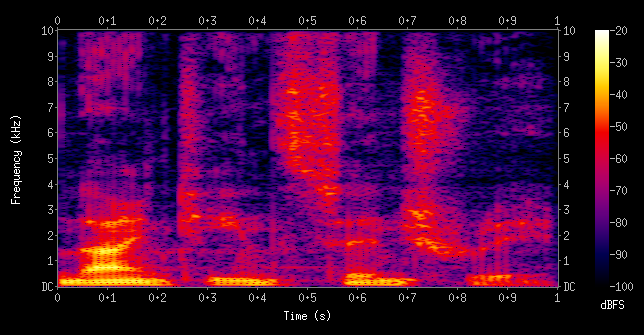
\includegraphics[width=0.75\textwidth]{BackgroundTheory/spectrogram.png}
    \captionof{figure}[Spectrogram]{Spectrogram of a spoken word phrase. It shows the time versus frequency relationship produced by the Fourier transform, as well as the intensity (amount) of each frequency for a time frame \cite{wiki:spectrogram}.}
    \label{fig:spectrogram}
\end{figure}

\subsection{Filters}
\label{subsec:filters}
During the processing of the audio signal we want to detect the frequency maxima
and minima of the wave, or possibly attenuate certain frequencies. In order to
do that we use \textit{audio filters} - tools that pass certain frequencies and
blocks others \cite{filters}. Filters are defined in terms of \textit{bands},
the range of frequencies they pass. A combination of filters which helps us
produce the required frequency cut-off is called a \textit{filter bank}.

\subsection{Scales}
\label{subsec:scales}
Earlier we mentioned that an octave contains 12 semitones. This is an
established standard - the semitones are equal on a logarithmic scale and form
the twelve-tone equal temperament or \textit{chromatic scale}. It is the
ordering that most Western music compositions employ and therefore the ordering
we use to determine relative positions in tones of audio signals. It is also the
scale which musical instruments often utilise. A good example of this are the
keys of a piano, which are ordered based on an equal temperament scale.

Another scale which is widely used to arrange values of a psychoacoustic
variable is the \text{mel scale}. It presents a perceptual ordering of pitches
which are determined to be equally far away from each other
\cite{stevens1937scale}. The scale introduces a unit of perceptual pitch called
\textit{mel}, where $1000\:mel = 1000\:Hz$. The rest of the mel-frequency
mapping is displayed in figure \ref{fig:melscale}. The conversion from $Hz$ to
$mel$ is calculated as:
\begin{figure}
    \begin{equation}
       Mel(f) = 2595\log{}(1 + \frac{f}{700})
    \end{equation}
    \captionof{figure}[Hz to mel conversion equation]{Converting a frequency of $f Hz$ into $mels$}
\end{figure}

\begin{figure}[H]
    \centering
    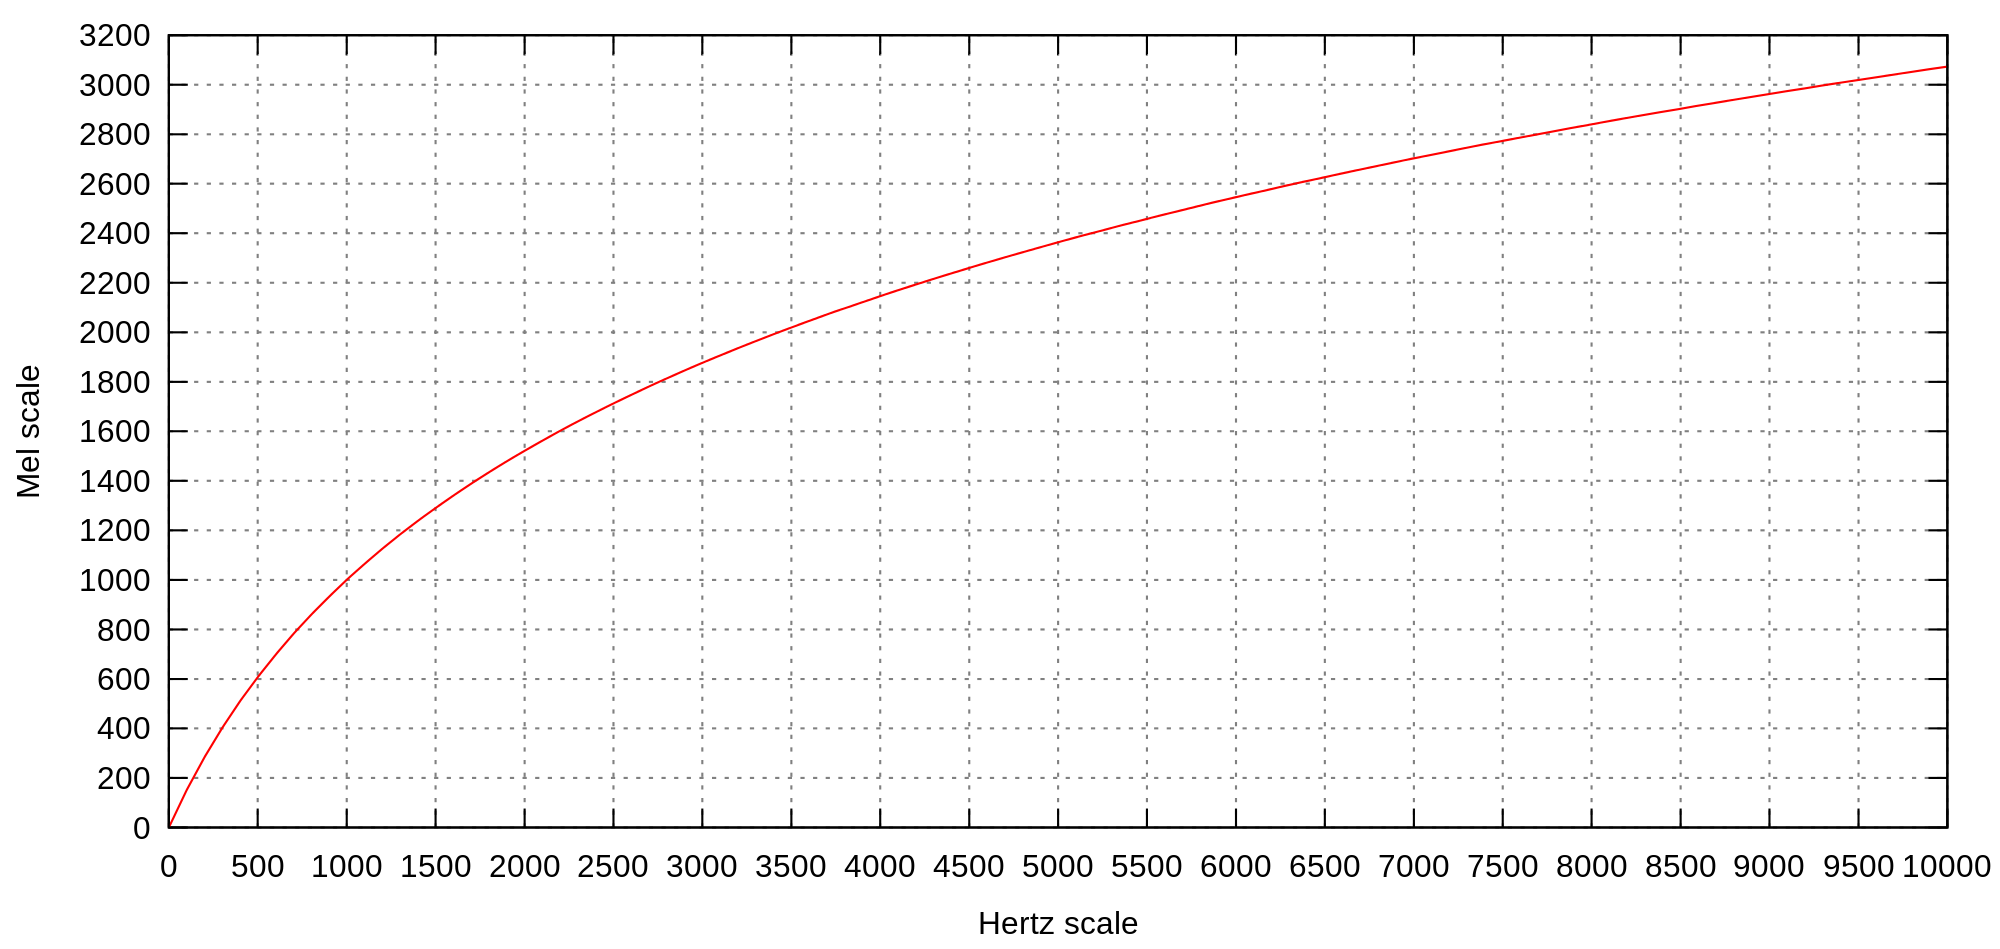
\includegraphics[width=0.85\textwidth]{BackgroundTheory/mel-scale.png}
    \captionof{figure}[Mel-scale]{Perceived pitches on a Mel scale versus the Hertz frequency scale \cite{wiki:melscale}}
    \label{fig:melscale}
\end{figure}

\section{Machine learning techniques}
\label{sec:machinelearning}
Some cover song identification algorithms create machine learning models based
on which they measure similarity when a query song is provided. This section
outlines the principles of each method used later in the algorithms.

\subsection{Random forests}
\label{subsec:randomforests}
Random forests are a form of ensemble learning for classification and regression
\cite{ho1995random}. Ensemble methods train multiple learners in an attempt to
solve the same problem \cite{zhou2012ensemble}, and in the case of random
forests the type of learner is a decision tree. The method works by building a
predefined number of decision trees during training, and return a result
combining their individual outcomes. In the case of classification the mode of
all returned class predictions is taken, while the mean of the predictions is
used during regression. 

Random trees learning generally builds upon the idea of recursive partitioning
used in decision tree learning. Partitioning builds a decision tree from the
training data based by asking questions related to the independent variables
(attributes) formed by the data samples. The 'answer' or split points for the
tree are called cut points. They are calculated to be the local optima values
which best split the data into homogenous sets based on the attribute. This
principle fails to create generalised models, since as the tree becomes deeper
and deeper the more it tends to overfit on their training data
\cite{friedman2001elements}.

Random trees help avoid the overfitting tendency of individual decision trees by
implementing bootstrap aggregating, also known as bagging. The learning
algorithm creates several small sets of uniformly sampled observations from the
training set and constructs trees using them. Depending on the configuration
some samples can be picked in more than one set. The end result is achieved
through the voting approaches explained above.

\subsection{K-means clustering}
\label{subsec:kmeansclustering}
K-means clustering is an unsupervised machine learning approach which aggregates
a collection of data points together because of some similarity between them.
The end result is a separation of the points into k distinct
clusters. The outcome of the clustering is evaluated through the sum of squares
defined as:
\begin{figure}[H]
   \begin{equation}
        Sum\;of\;squares = \sum_{i=1}^{n}(x_i - \overline{x})^2
   \end{equation} 
   \captionof{figure}[Sum of squares equation]{The sum of squares for $n$ items where $x_i$ is the value of the i-th item and $\overline{x}$ is the mean of the set $n$.}
   \label{fig:sumofsquares}
\end{figure}

The intent is to reduce the sum of squares as much as possible. Clustering is
complete when either the sum of squares does not significantly change any more,
or the algorithm runs a pre-determined number of iterations.

In the area of digital signal processing K-means clustering is used to perform 
\textit{quantisation} - mapping a large (possibly continuous) set of values to a
countable smaller set which is easier to work with \cite{wiki:quantisation}.


% add more sections and subsection here
